\documentclass[12pt]{article}
\usepackage{hyperref}
\usepackage[authoryear, round,sort,comma,numbers]{natbib}
\usepackage{times}
\usepackage{color}
\usepackage{apalike}
\usepackage{graphicx}
\usepackage{authblk}
\usepackage{amsmath}



%\usepackage[maxbibnames=99]{biblatex}
%\usepackage{setspace}
%\usepackage{geometry}
\usepackage[font={sf,small}]{caption}
%\usepackage{setspace}
%\usepackage{geometry}
%\usepackage{hyperref}
%\hypersetup{
%    colorlinks,
%    citecolor=black,
%    filecolor=black,
%    linkcolor=black,
%    urlcolor=black
%}
%\geometry{letterpaper}

\usepackage{amssymb}
%\usepackage{epstopdf}
\usepackage{float}
%\DeclareGraphicsRule{.tif}{png}{.png}{`convert #1 `dirname #1`/`basename #1 .tif`.png}

\newcommand{\specialcell}[2][c]{%
	\begin{tabular}[#1]{@{}c@{}}#2\end{tabular}}
\setlength{\textheight}{9.3in}
\setlength{\textwidth}{7in}
\setlength{\footskip}{0.5in}
\setlength{\topmargin}{-0.5in}
\setlength{\headheight}{0.2in}
\setlength{\headsep}{0in}
\setlength{\parindent}{1pc}
\setlength{\oddsidemargin}{-0.25in}
\setlength{\evensidemargin}{-0.25in}
\renewcommand{\baselinestretch}{1.5}


\title{What is the nature of decision noise in random exploration?}

\author[1]{Siyu Wang}
\author[1,2]{Robert C. Wilson}


\affil[1]{Department of Psychology, University of Arizona, Tucson AZ USA}
\affil[2]{Cognitive Science Program, University of Arizona, Tucson AZ USA}


\date{\today}

\begin{document}
	\maketitle
	
	\newpage
	\begin{abstract}
	[150 words for Nature Human Behavior, currently 162]
	Human decision making appears to contains components that are inherently random. While this behavioral variability has traditionally been seen as noise, recent work suggests that random choices may actually be adaptive. An example arises when deciding between exploring unknown options or exploiting options we know well. Theory shows that a little randomness in explore-exploit decisions is remarkably effective, leading to greater rewards overall. Meanwhile, experiments show that people use such `random exploration' in practice,  increasing their behavioral variability when it is more valuable to explore. Despite this progress, the nature of adaptive decision noise is unknown and it is unclear whether it is generated internally, from stochastic processes in the brain, or externally, from stochastic stimuli in the world? Here we show that, while both types of noise are present in explore-exploit decisions, random exploration is dominated by internal noise. This suggests that random exploration depends on adaptive noise processes in the brain which are subject to (perhaps unconscious) cognitive control.
	
	%From everyday decisions, like deciding where to dine, to major life milestones, like deciding whom to marry, many decisions involve a tradeoff between exploring options that are unknown and exploiting options we know well. 
	
	%Recently we have shown that humans make simple explore-exploit choices using two distinct strategies. One of these strategies, known as random exploration, involves choice randomization
	
	%While making optimal explore-exploit choices is a hard computational problem, we have recently shown that humans make effective explore-exploit choices using heuristic strategies. One particularly simple strategy is `random exploration'.  In this strategy, the decision process is noisy meaning that high value `exploit' options are not always chosen and exploratory choices are sometimes made by chance. 
	
	%Despite this progress, questions remain about the nature of random exploration in particular, is the noise in behavior generated internally, from stochastic processes in the brain, or externally, from stochastic stimuli in the world?
	
	%as there are a number of ways in which seemingly stochastic choices could be generated. In one strategy, the `external noise strategy,' participants could rely on stochasticity in the world and allow irrelevant features of the stimulus to drive choice. In another strategy called `internal noise strategy,' people could rely on stochastic processes within their own brains. 
	
	%In this work, we modified our recently published `Horizon Task' in such a way as to distinguish these two strategies. Using both a model-free and model-based analysis of human behavior we show that, while both types of noise are present in explore-exploit decisions, random exploration is dominated by internal noise. This suggests that random exploration depends on adaptive noise processes in the brain which are subject to (perhaps unconscious) cognitive control. 
	\end{abstract}
	\newpage
	
	%In theory, such `random exploration', can be surprisingly effective in explore-exploit problems and, if implemented correctly, can come close to optimal performance.
	%Moreover, recent work suggests that humans actually use random exploration in simple explore-exploit tasks. 
	
	\section*{Introduction}
	
	Imagine trying to decide where to go to dinner with a friend. You can go to your favorite restaurant that you both really enjoy and always go to, or you can try the new restaurant that just opened and about which you know nothing. Such decisions, in which we must choose between a well-known exploit option and a lesser known explore option, are known as explore-exploit decisions.  From a theoretical perspective, making optimal explore-exploit choices, i.e. choices that maximize long-term reward, is incredibly hard \citep{eegittins74} (CITE BELMAN). In part because of this difficulty, there is considerable interest in how humans and animals solve the explore-exploit dilemma in practice \citep{, eeauer02,eegittins79,eekrebs78,eethompson33, eewatkins89, eebridle90,eemeyer95, eebanks97,eefrank09, eesteyvers09, eelee11, eepl12,eezhang13,eedaw06, eepl11, wilson2014}.
	
	One particularly effective strategy for solving the explore-exploit dilemma is choice randomization \citep{eethompson33, eewatkins89, eebridle90}. In this strategy, the decision process between exploration and exploitation is corrupted by `decision noise', meaning that high value `exploit' options are not always chosen and exploratory choices are sometimes made by chance. In theory, such `random exploration,' is surprisingly effective and, if implemented correctly, can come close to optimal performance \citep{eebridle90} CITE THOMPSON AND NEW PAPERS ON THOMPSON SAMPLING. 
	
	Recently we have shown that humans appear to actually use random exploration and actively adapt their decision noise to solve simple explore-exploit problems \citep{wilson2014}.  The key manipulation in the task is the horizon condition, i.e. the number of decisions remaining to make. Increasing the horizon makes exploration more valuable as there is more time to use the information gained by exploration to maximize future rewards. For example, if you are leaving town tomorrow (short horizon), you will probably exploit the restaurant you know and love, but if you are in town for a while (long horizon), you would be more likely to explore the new place. Using such a horizon manipulation we found that people have greater decision noise in the long versus the short horizon condition. 
	
	
	However, a key limitation of this work was that the source of the decision noise used for exploration is unknown. Of particular interest is whether the adaptive decision noise that is linked to exploration arises externally, in the input from the world, or is generated internally, within the brain. In the restaurant case, an example of external noise would be if you happen to spot an old friend walking in to one of the restaurants. Conversely, internal noise would arise from stochastic neural processes tossing a metaphorical coin in your head. Previous work makes a strong case for both types of noise being relevant to behavior. For instance, external, stimulus-driven noise is thought to be a much greater source of choice variability in perceptual decisions than internal noise \citep{eeBrunton13}. Conversely internal, neural noise is thought to drive exploratory singing behavior in song birds  \citep{songbird2} and the generation and control of this internal noise has been linked to specific neural structures CITES. 
	
	In this paper, we investigate which source of noise, internal vs external, drives random exploration in humans in a simple explore-exploit task adapted from our previous work \citep{wilson2014}. To distinguish between the two types of noise, we had people make the exact same explore-exploit decision twice. If decision noise is purely externally driven, then people's choices should be identical both times, that is their choices should be consistent, since the stimulus is the same both times. Meanwhile, if noise is internally driven their choices should be inconsistent, since the internal noise is different both times. By analyzing behavior on this task in both a model-free and model-based manner, we show that, while both types of noise are present in explore-exploit decisions, the contribution of internal noise to random exploration far exceeds that contributed by the stimulus.
	
	
	%\begin{figure}[H]
	%	\begin{center}
	%		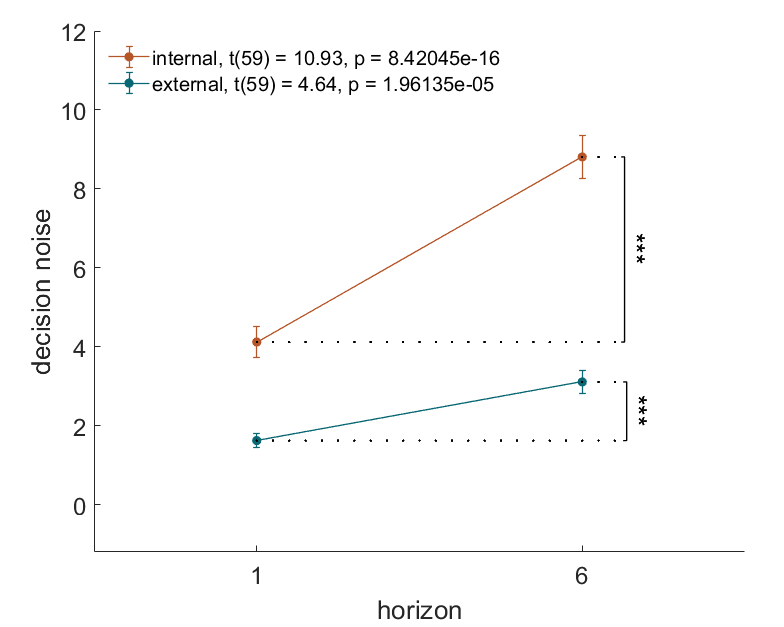
\includegraphics[width=0.7\textwidth]{figs/bayes_s.png}
	%			\caption[Subject level estimated mean of external and internal noise variance.]{Subject level estimated mean of external and internal noise variance. Both internal and external noise increase with horizon, internal noise is dominant.}
	%			\label{fig:mb3}
	%		\end{center}
	%	\end{figure}
	
	
	
	\section*{Results}
	
	\subsection*{The Repeated-Games Horizon Task}
	We used a modified version of the `Horizon Task' \citep{wilson2014} to show the influence of internal vs external noise on people's decisions (Figure \ref{fig:taskfig}). In this task, participants make repeated choices between two slot machines, or `one-armed bandits,' that pay out probabilistic rewards. Because they are initially unsure as to the mean payoff of each bandit, this task requires that participants carefully balance exploration of the lesser known bandit with exploitation of the better known bandit to maximize their overall rewards. 
	
	Crucially, before people make their first choice in the Horizon Task, they are given information about the mean payoff from each bandit, in the form of four example plays distributed either unequally between bandits (i.e. 1 play of one bandit, 3 plays of the other) or equally (2 plays each). These example plays allow us to manipulate exactly what people know about each option before they make their first choice. Thus, by giving people the exact same example plays twice in two separate games (separated by several minutes in time so as to avoid detection), the example plays allow us to probe how participants respond to the exact same explore-exploit choice twice.  
	
	These `repeated games' are the key manipulation in this paper and allow us to distinguish between external and internal sources of noise.  Specifically, if noise is externally driven, then choices on repeated games should be consistent. Conversely if noise is internally driven, then choices on repeated games should be inconsistent.
	
	\begin{figure}[h]
		\begin{center}
			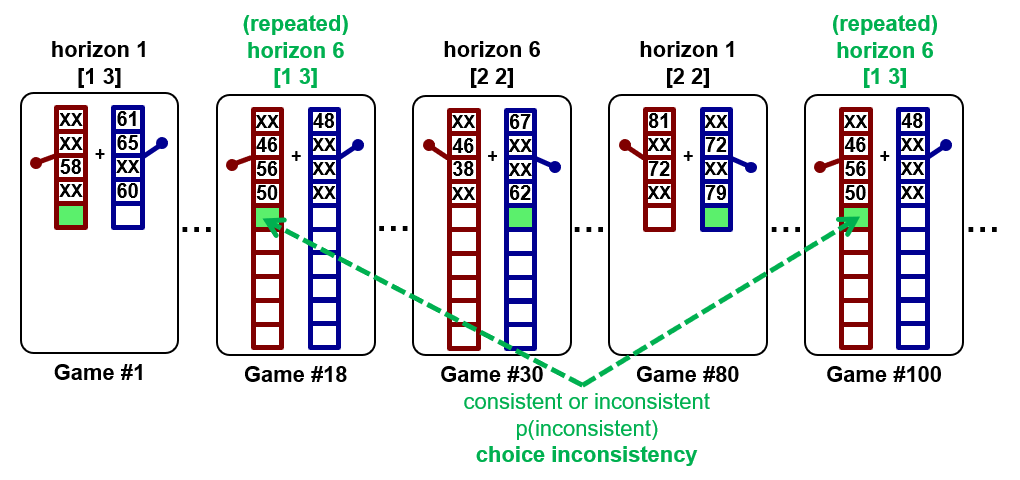
\includegraphics[width=\textwidth]{figures/taskfig.PNG}
			\caption{A key additional manipulation here is repeated games. Each pair of repeated games with identical example trials will appear twice during the experiment. We setup the repeated games such that they are at least 5 games apart from each other. A model-free measure of choice inconsistency which reflex the underlying decision noise is defined as the proportion of inconsistent choices for repeated games.}
			\label{fig:taskfig}
		\end{center}
	\end{figure}
	
	\subsection*{Both behavioral variability and information seeking increase with horizon}
	
	%This further allowed us to have people make the exact same
	
	%The key manipulation was to use repeated games to let people make the same decision twice. In the restaurant example, if your decision is mainly driven by external noise, then a few months later when you see the friend walking in front of you into the restaurant, you are very likely to make the same decision and follow him into that restaurant to say hi. However, if your decision is mainly driven by internal noise, then next time you make a split-second decision about where to go, you are equally likely to go to the other restaurant.
	
	%More specifically, we look at the contribution of external and internal noise by providing with participants the same decision problem twice in the task. In this task, participants play a set of games in which they make choices between two slot machines (one-armed bandits) that pay out rewards from different Gaussian distributions. To maximize their rewards in each game, participants need to exploit the slot machine with the highest mean, but they cannot identify this best option without exploring both options first. 
	
	%In each game they made multiple decisions between two options. Each option paid out a random reward between 1 and 100 points sampled from a Gaussian distribution. The means of the underlying Gaussian were different for the two bandit options, remained the same within a game, but changed with each new game. One of the bandit will always have a higher mean than the other. Participants were instructed to maximize the points earned over the entire task.
	
	%The first four trials of each game were forced-choice trials, in which only one of the options was available for the participant to choose. We used these forced-choice trials to manipulate the relative ambiguity of the two options, by providing the participant with different amounts of information about each bandit before their first free choice. The four forced-choice trials set up two uncertainty conditions: unequal uncertainty(or [1 3]) in which one option was forced to be played once and the other three times, and equal uncertainty(or [2 2]) in which each option was forced to be played twice. After the forced-choice trials, participants made either 1 or 6 free choices (two horizon conditions). In unequal uncertainty condition, people are more likely to choose the option that they know less about - the more informative option - to explicitly explore that option more. This type of information driven exploration is known as directed exploration.
	
	Before discussing the results for repeated games, we first confirm that the basic behavior in this task is consistent with our previously reported results \citep{wilson2014}. As in our previous work, we find evidence for two types of exploration in the Horizon Task.  Random exploration, which is the main focus of this paper, where exploration is driven by noise, and directed exploration, where exploration is driven by information. 
	
	Random exploration is quantified in a model-free way as the probability of choosing the low mean option, $p(\mbox{low mean})$ in the equal, or [2 2], condition. This value increases with horizon, consistent with the idea that behavior is more random in horizon 6 (t(59) = 6.17, p $<$ 0.001 for [1 3], t(59) = 7.26, p $<$ 0.001 for [2 2]).  Directed exploration, is measured as the probability of choosing the more informative option $p(\mbox{high info}$ in the unequal, or [1 3], condition. Again this measure increases with horizon, showing that people are more information seeking in horizon 6 (t(59)=6.88, p $<$ 0.001).
	
	%These conditions allow us to measure directed and random exploration in a model-free way. Directed exploration is measured as the probability of choosing the more informative option in [1 3] condition whereas random exploration is measured as the probability of choosing the low mean option in [2 2] condition. In line with previous results \citep{wilson2014}, we showed that both directed and random exploration increase with horizon. Both direct (t(59)=6.88, p $<$ 0.001) and random exploration (t(59) = 6.17, p $<$ 0.001 for [1 3], t(59) = 7.26, p $<$ 0.001 for [2 2]) increases with horizon. (Figure \ref{fig:modelfree}, A,B).   Directed exploration is considered to be driven by information bias and random exploration is considered to be driven by decision noise, in this work, we are investigating which source of decision noise, external vs internal, drives random exploration.
	
	%the influence of directed exploration is measured as the probability of choosing the more informative option, i.e. the bandit with only 1 outcome in [1 3] condition; decision noise is measured as the probability of choosing the low mean option in [2 2] condition.
	
	
	
	\begin{figure}[H]
		\begin{center}
			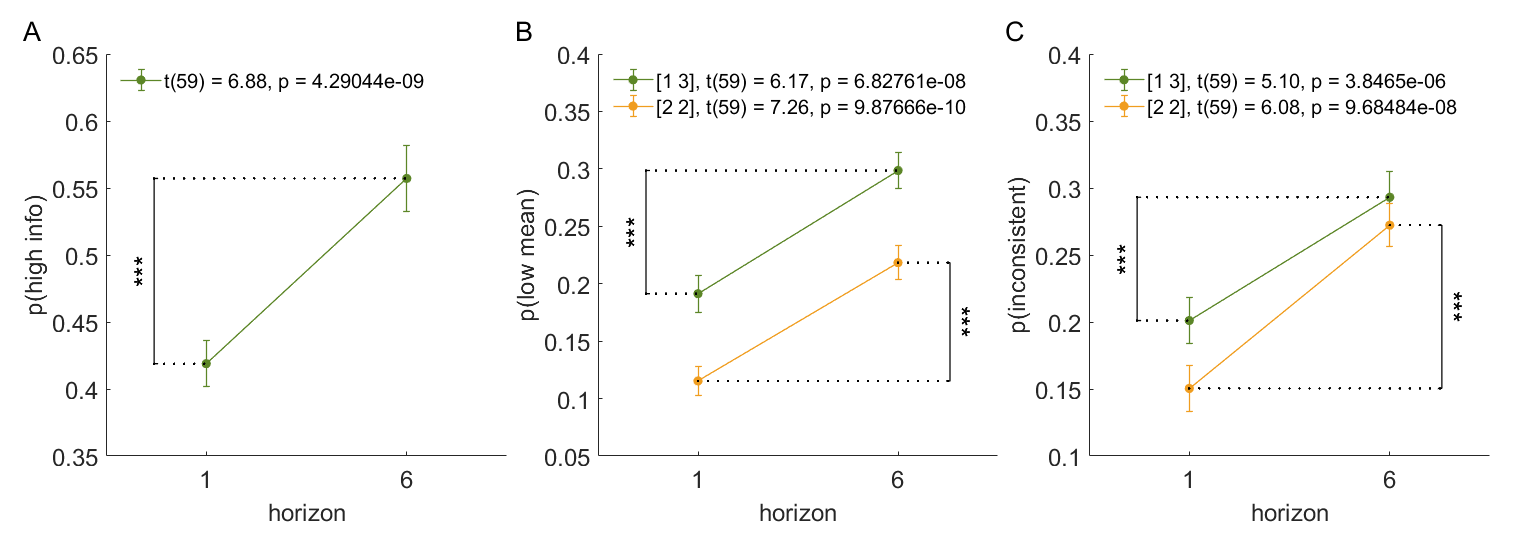
\includegraphics[width=\textwidth]{figures/modelfree.png}
			\caption{Both directed and random exploration increase with horizon. Choice inconsistency also increases with horizon for both [1 3] and [2 2] conditions. TAKE OUT PANEL C }
			\label{fig:modelfree}
		\end{center}
	\end{figure}
	
	%Finally, the crucial additional manipulation in this task is repeated games (Figure \ref{fig:taskfig}). In each pair of repeated games, the four forced-choice trials were yoked, meaning that on the first free choice trial participants were faced with identical stimuli.  After the first free choice trial, the outcomes on the repeated games were not yoked and the outcomes were sampled independently from the underlying Gaussian distribution.  Not yoking the later trials made it harder for participants to detect repeated games.  In addition, the presentation of repeated games was controlled so that each repeated pair was at least five games away from each other. 
	
	\subsection*{Model-free analysis shows that random exploration may involve both internal and external noise}
	
	%In this section we use both model-free and model-based analyses to show that both internal and external noise contribute to the behavioral variability in random exploration. Using the model-based hierarchical Bayesian analysis, we also show that the effect of internal noise is the main source of noise in random exploration.
	
	%\subsubsection*{Model-free analysis}
	Next we asked whether participants' choices were consistent or inconsistent in the two repetitions of each game.  The idea behind this measure is that purely external noise should lead to consistent choices as the external stimulus is identical both times. Conversely, purely internal noise should lead to independent choices, and hence more inconsistent choices both times. 
	
	To quantify choice inconsistency we computed the frequency with which participants made different responses for pairs of repeated games (Figure \ref{fig:mf2}). Using this measure we found that participants made inconsistent choices in both the unequal ([1 3]) and equal ([2 2]) information conditions (STATS), suggesting that not all of the noise was stimulus driven. In addition, we found that choice inconsistency was higher in horizon 6 than in horizon 1 for both [1 3] and [2 2] condition (STATS ANOVA WITH HORIZON AND UNCERTAINTY CONDITIONS AS FACTORS), suggesting that at least some of the horizon dependent noise is internal.
	
	
	%As is clear from the plots, in both the unequal ([1 3], panel A) and equal ([2 2], panel B) conditions, 
	
	%In addition, whether participants make consistent choices in repeated games is used as a model-free measure of internal noise, since in repeated trials, external noise should be identical on both trials. So only internal noise can differ and drive the choice inconsistency. The degree to which people make consistent choices in repeated trials can reflect the internal noise.  Since choice inconsistency in both [1 3](t(59) = 5.10, P([1 3]) $<$ 0.001) and [2 2](t(59) = 6.08, P([2 2])$<$0.001) condition increase with horizon (Figure \ref{fig:modelfree} C), this is a behavioral evidence that internal noise increases with horizon.
	
	%Choice inconsistency between repeated games was non-zero in both horizon conditions, suggesting that not all of the noise was stimulus driven.  In addition, choice inconsistency was higher in horizon 6 than in horizon 1 for both [1 3] and [2 2] condition (Figure \ref{fig:modelfree}), suggesting that at least some of the horizon dependent noise is internal.
	
	\begin{figure}[h]
		\begin{center}
			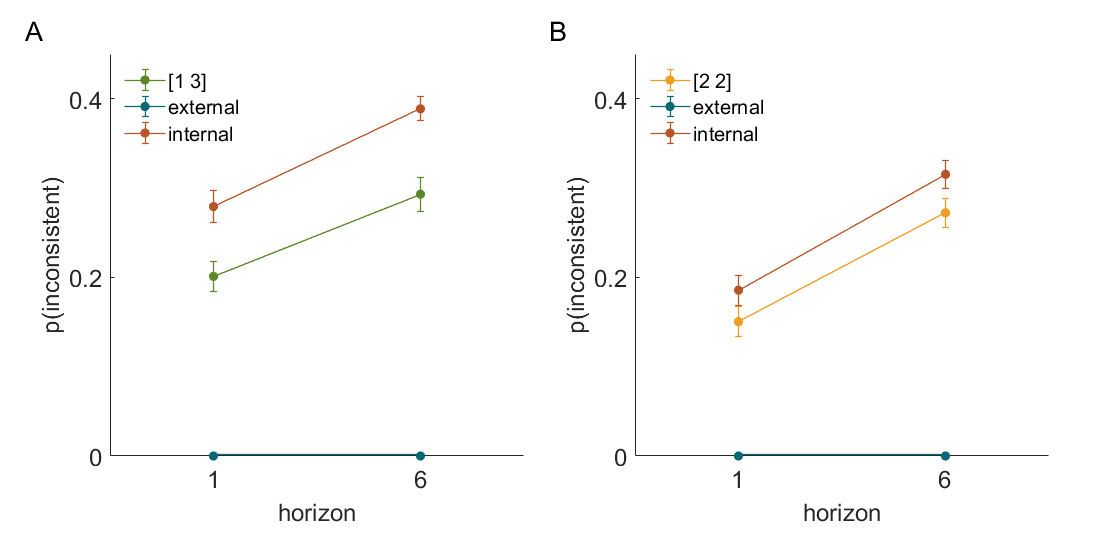
\includegraphics[width=\textwidth]{figures/modelfree_intext.png}
			\caption[Both external and internal noise contribute to the choice variability in random exploration]{Both external and internal noise contribute to the choice variability in random exploration. For both [1 3] and [2 2] condition, there is a significant difference between people's behavior and predicted choice inconsistency assuming that only external noise exists where people should behave identically in repeated games. Also, there is a significant difference between people's behavior and predicted choice inconsistency assuming that only internal noise exists where people treat repeated games independently. }
			\label{fig:mf2}
		\end{center}
	\end{figure}
	
	To gain more quantitative insight into these results, we computed theoretical values for the choice inconsistency for the purely external and purely internal noise cases.  For purely external noise this computation is simple because people should make the exact same decisions each time in repeated games, meaning that $p(\mbox{inconsistent}) = 0$ in this case. For purely internal noise, the two games should be treated independently, allowing us to compute the choice inconsistency in terms of the probability of choosing the low mean option, $p(\mbox{low mean})$, as
	\begin{equation*}
	\begin{split}
	p(\mbox{consistent}) &= p(\mbox{low mean})^2 + p(\mbox{high mean})^2\\
	&= p(\mbox{low mean})^2 + (1-p(\mbox{low mean}))^2\\ 
	\mbox{hence},\quad p(\mbox{inconsistent}) &=  2 p(\mbox{low mean}) CHECK????
	\end{split}
	\end{equation*}
	As shown in Figure  \ref{fig:mf2}, people's behavior falls in between the pure external noise prediction and the pure internal noise prediction (STATS T-TEST RELATIVE TO BOTH), suggesting that both external and internal noise are present in driving this choice inconsistency. Since choice inconsistency only reflects internal noise, Figure \ref{fig:mf2} suggests that internal noise increases with horizon.
	
	\subsection*{Model-based analysis shows that random exploration is dominated by internal noise}
	
	To more precisely quantify internal and external noise, we turned to model fitting. We modeled behavior on the first free choice of the Horizon Task using a version of the logistic choice model in \citep{wilson2014} that was modified to differentiate internal and external noises. In particular, we assume that in repeated games, external noise remains the same whereas internal noise can change. 
	
	\subsubsection*{Overview of model}
	As with our model-free analysis, the model-based analysis focuses only on the first free-choice trial since that is the only free choice when we have control over the information bias between the two bandits. To model participants' choices on this first free-choice trial, we assume that they make decisions by computing the difference in value $\Delta Q$ between the right and left options, choosing right when $\Delta Q > 0$ and left otherwise.  Specifically, we write
	\begin{equation}
	\Delta Q= \Delta R+A \Delta    I+b+n_{ext}+n_{int}
	\end{equation}
	where, the experimentally controlled variables are $\Delta R=R_{right}-R_{left}$, the difference between the mean of rewards shown on the forced trials, and $\Delta I$, the difference information available for playing the two options on the first free-choice trial. For simplicity, and because information is manipulated categorically in the Horizon Task, we define $\Delta I$ to be +1, -1 or 0, +1 if one reward is drawn from the right option and three are drawn from the left in the [1 3] condition, -1 if one from the left and three from the right, and in [2 2] condition, $\Delta I$ is 0. $n_{ext}$ and $n_{int}$ are external noise and internal noise respectively.
	
	The subject-and-condition-specific parameters are: the spatial bias, $b$, which determines the extent to which participants prefer the option on the right; the information bonus $A$, which controls the level of directed exploration; $n_{ext}$ denotes the external, external noise, which is identical on the repeat versions of each game; and $n_{int}$ denotes internal noise, which is uncorrelated between repeat plays and changes every game.
	
	For each pair of repeated games, the set of forced-choice trials are exactly the same, so the external noise, $n_{ext}$, should be the same while the internal noise, $n_{int}$ may be different. This is exactly how we distinguish external noise from internal noise. In symbolic terms, for repeated games $i$ and $j$,  $n_{ext}^i=n_{ext}^j$  and $n_{int}^i \neq n_{int}^j$.
	
	
	\subsubsection*{Model fitting}
	We used hierarchical Bayesian analysis to fit the parameters of the model (see Figure \ref{fig:model} for an graphical representation of the model in the style of \cite{lee2014}). In particular, we fit values of the information bonus $A$, spatial bias $B$, variance of internal noise $\sigma_{int}^2$, and variance of external noise, $\sigma_{ext}^2$ for each participant in each horizon. Model fitting was performed using the MATJAGS and JAGS software \citep{jags, matjags} with full details given in the Methods.   %The mean and standard deviation of information bonus $A$ and spatial bias $B$ are sampled from a Gaussian prior and an exponential prior respectively. The variance for both type of noises were sampled from a gamma distribution, and the group-level parameter $k$ and $\lambda$ for the gamma distribution are sampled from exponential priors. 
	
	%To capture the idea that external noise should be identical on repeated games, we sampled one value of the external noise, $n_{ext}$ for each pair of repeated games.  Conversely, because internal noise is expected to change between games we sampled two values of the internal noise, $n_{int}^1$ and $n_{int}^2$, i.e. one for each individual game.  
	
	%The model in Figure \ref{fig:model} is fitted using the MATJAGS and JAGS software \citep{jags, matjags}.
	
	
	%Before presenting the results of the model-based analysis we begin with a brief overview of the most salient points of the model.  A full description of the model can be found in the Methods and code to implement the model can be found in the Supplementary Material.  
	
	%Conceptually, the model breaks the explore-exploit choice down into two components: a learning component, in which participants estimate the mean payoff of each option from the rewards they see, and a decision component, in which participants use this estimated payoff to guide their choice.  The learning component assumes that participants compute an estimate of the average payoff for each slot machine, $R^i_t$, using a simple delta rule update equation (based on a Kalman filter \cite{Kalman1960-uo}, see Methods):
	%\begin{equation}
	%R^i_{t+1}= R^i_t + \alpha_t^i (r_t - R^i_t)
	%\end{equation}
	%where $r_t$ is the reward on trial $t$ and $\alpha_t^i$ is the time-varying learning rate that determines the extent to which the prediction error, $(r_t - R^i_t)$, updates the estimate of the mean of bandit $i$. The learning process is described by three free parameters: the initial value of the estimated payoff, $R_0$, and two learning rates, the initial learning rate, $\alpha_1$, and the asymptotic learning rate, $\alpha_{\inf}$, which together describe the evolution of the actual learning rate, $\alpha_t$, over time. For simplicity, we assume that these parameters are independent of horizon and uncertainty condition (Table 1).
	
	%The decision component of the model assumes that participants choose between the two options (left and right) probabilistically according to 
	%\begin{equation}
	%	p(\mbox{choose right}) = \frac{1}{ 1 + \exp \left( \frac{\Delta R + A \Delta I + B}{\sigma}\right) }
	%\end{equation}
	%where $\Delta R$ ( $= R^{left}_t - R^{right}_t$ ) is the difference in expected reward between left and right options and $\Delta I$ is the difference in information between left and right options (which we define as +1 when left is more informative, -1 when right is more informative, and 0 when both options convey equal information in the [2 2] condition). The decision process is described by three free parameters: the information bonus $A$, the spatial bias $B$, and the decision noise $\sigma$.  We estimate separate values of the decision parameters for each horizon and (since the information bonus is only used in the [1 3] condition) separate values of only the bias and decision noise for each uncertainty condition. 
	
	
	
	
	
	%Overall, subject's behavior in each session (vertex vs RFPC stimulation) is described by 13 free parameters (Table \ref{table1}): three describing learning ($R_0$, $\alpha_1$ and $\alpha_{\infty}$) and 10 describing the decision process ($A$ in the two horizon conditions, $B$ and $\sigma$ in the four horizon-x-uncertainty conditions). These 13 parameters were fit to each subject in each stimulation condition using a hierarchical Bayesian approach \cite{Lee2014-yh} (see Methods).  
	
	\subsubsection*{Model fitting results} 
	
	%Group-level estimates for the variances of internal and external noise are shown in Figure \ref{fig:modelbased}A.  While both variances are non-zero, this shows that the internal noise is much larger than external noise. This horizon-based change is probed further in Figure XXXB in which we plot the posterior distributions over the change in internal and external noise with horizon.  This clearly shows that only internal noise varies with horizon (STATS XXX\% of the samples above zero for internal noise, XXX\% of samples above zero for external noise).
	
	Posterior distributions over the group-level means of the external and internal noise variance are shown in Figure \ref{fig:mb1}. Consistent with our model-free results, we see that both internal and external noise variances are non-zero and that internal noise is about 2-3 times larger than the external noise. In addition, we find that internal noise increases dramatically with horizon (STATS) whereas there is only a slight increase of external noise (STATS).  Taken together, these results suggest that random exploration is dominated by internal noise.
	
	%internal noise changes 
	
	%appear to increase with horizon (Figure \ref{fig:mb2}, 100\% of the samples above zero for internal noise, 96.33\% of samples above zero for external noise), the change in internal noise is much larger (STATS).
	
	%With regard to the change in noise between horizons, 
	
	%While both variances are non-zero, this shows that the internal noise is much larger than external noise. This horizon-based change is probed further in Figure \ref{fig:mb2} in which we plot the posterior distributions over the change in internal and external noise with horizon. As is clear from this plot, internal noise increases dramatically with horizon whereas there is a slight increase of external noise with horizon as well (0 just falls in the critical region at level of 5\% for external noise but lies right at the border, although significant, it's not as strong as the internal noise). This clearly shows that internal noise dominates and significantly varies with horizon  (100\% of the samples above zero for internal noise, 96.33\% of samples above zero for external noise). 
	
	%Furthermore, we plotted the subject level estimates of both internal and external noises in a similar fashion of the model-free plot of choice-inconsistency for comparison (Figure \ref{fig:mb3}). We showed again that both internal and external noises increase significantly with horizon. But in terms of magnitude, internal noise is what' really dominant here (See also Figure \ref{fig:rcurvepd6} in Appendix \ref{ch:appendicies:reward}). Subject-level estimates also allow us to look at the relationship between internal and external noises, and we showed that internal noise correlates with external noise significantly in both horizon conditions ($R^2 = 0.32, p < 0.001$ in horizon 1, $R^2 = 0.24, p < 0.001$ in horizon 6, see Figure \ref{fig:corrintext} in Appendix \ref{ch:appendix:corrintext}).
	
	
	\begin{figure}[h]
		\begin{center}
			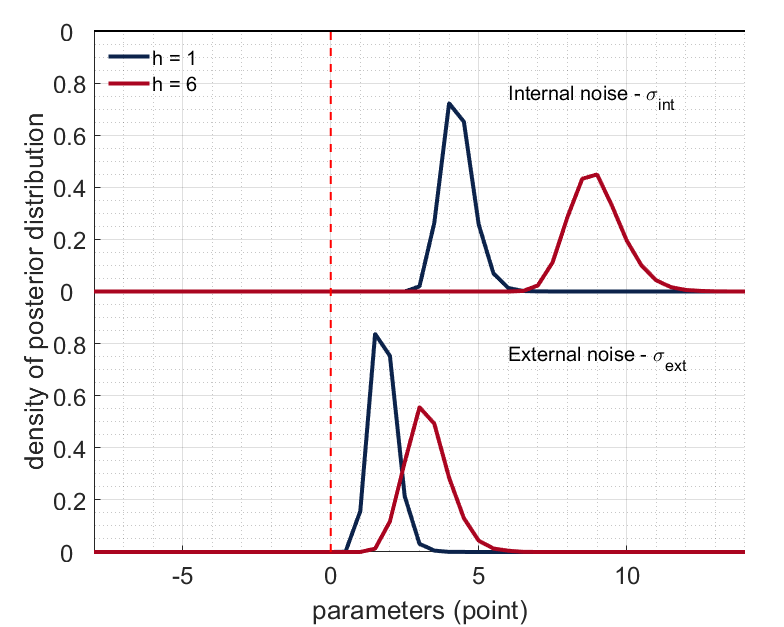
\includegraphics[width=0.7\textwidth]{figures/dist_hypernoiseh.png}
			\caption[Posterior distributions over the group-level means of the external and internal noise variance.]{Posterior distributions over the group-level means of the external and internal noise variance. Both internal and external noises are nonzero, and internal noise has a much greater magnitude. COMBINE FIGURES 4 AND 5, USE SEPARATE PANELS FOR EACH ONE, REMOVE INCORRECT RED SHADED REGION ON TOP PANEL OF FIGURE 5, Y-AXIS CAN BE LABELED 'posterior density' X-AXIS IS 'noise standard deviation [points]'}
			\label{fig:mb1}
		\end{center}
	\end{figure}
	
	
	%LEFT EACH TYPE OF NOISE IN EACH HORIZON
	%RIGHT IS DISTRIBUTION OVER CHANGE IN NOISE WITH HORIZON
	
	%Posterior distributions over the group-level means of the external and internal noise variance are shown in Figure \ref{fig:modelbased}.  As is clear from this plot, only internal noise increases  with horizon. 
	%In both horizon 1 and horizon 6, internal noises are significantly higher than internal noises (for both horizon 1 and horizon 6, P $<$ 0.001).
	
	
	\begin{figure}[H]
		\begin{center}
			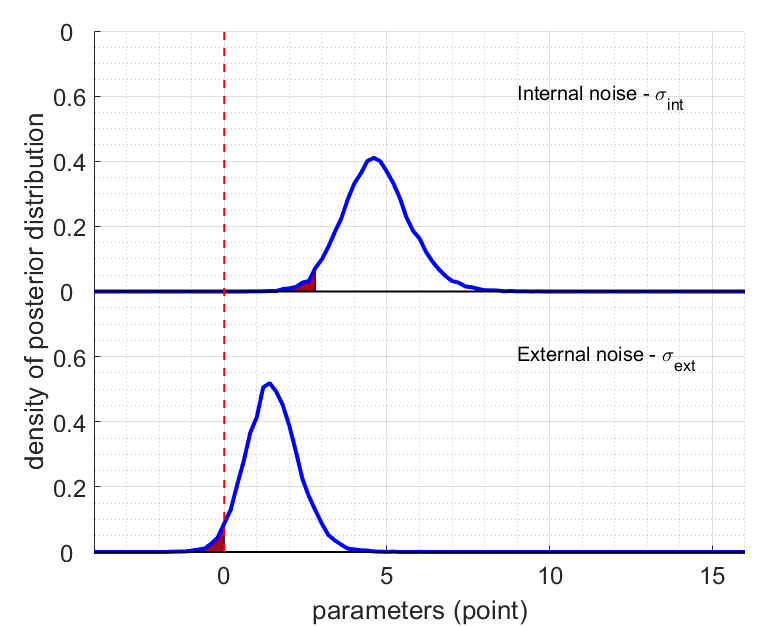
\includegraphics[width=0.7\textwidth]{figures/dist_hypernoise.png}
			\caption[Posterior distributions over the group-level means of the change of external and internal noise variance.]{Posterior distributions over the group-level means of the change of external and internal noise variance. Internal noise increases significantly with horizon, external noise increases with horizon as well.}			
			\label{fig:mb2}
		\end{center}
	\end{figure}
	
	\section*{Discussion}
	In this paper, we investigated whether random exploration is driven by internal noise, putatively arising in the brain, or external noise, arising from the environment. Using a version of the Horizon Task with repeated games, we found that evidence for both types of noise in explore-exploit decisions. In addition, we see that both internal and external noise increase with horizon, but that the horizon effect is much larger for internal noise.  Taken together our results suggest that random exploration, i.e. the use and adaptation of decision noise to drive exploration, is driven primarily by internal noise.

	Perhaps the main limitation of this work is in the interpretation of the different types of noise as being internal and external. In particular, while we controlled many aspects of the stimulus across repeated games (e.g. the outcomes and the order of the forced trials), we could not perfectly control {\it all} stimuli the participant received, which would vary, for example, based on exactly what they were looking at or whether they were scratching their nose. Thus, our estimate of external noise is likely a lower bound. Likewise, our estimate of internal noise is likely an upper bound as these `missing' sources of external noise would be interpreted as internal noise in our model. Despite this, it seems hard to imagine that these additional noise sources could be enough to account for the large differences between internal and external noise that we found in Figure \ref{fig:mb2}, where internal noise is 2-3 times the size of external noise.  
	
	Taken at face value, the horizon-dependent increase in internal noise is consistent with the idea that random exploration is driven by intrinsic variability in the brain. This is in line with work in the bird song literature in which song variability during song learning has been tied to neural variability arising from specific areas of the brain \citep{songbird1, songbird2}. In addition, this work is consistent with a recent report from \cite{ebitz17} in which the behavioral variability of monkeys in an `explore' state was also tied to internal rather than external sources of noise. 
	
	Whether such a noise-controlling area exists in the human brain is less well established, but one candidate theory \citep{aj2005} suggests that norepinephrine (NE) from the locus coeruleus may play a role in modulating internal levels of noise. Indeed, manipulation of the NE system has been found to change behavioral variability in both humans and other animals in a variety of tasks (CITES KARPOVA, PAPER I JUST SENT YOU AND REFS WITHIN, ALSO JANE'S BIOARXIV PAPER).  In addition there is some evidence that NE plays a direct role in random exploration (CITE WARREN ET AL. 2017), although this finding is complicated by other work showing no effect of NE drugs on exploration CITE NIEWENHUIS AND JEPMA DRUG STUDY.

	More generally, our finding that internal noise dominates behavioral variability over external noise, is consistent with findings of \cite{drugowitsch16}. In particular these authors show that randomness in behavior arises from imperfections in mental inference, that happen inside the brain, rather than in peripheral processes such as sensory processing and response selection. This suggests that most noise in behavior is generated internally and that this may arise from  computational errors in computing the correct strategy. In the context of the Horizon Task, such computational errors would likely be larger  in the long horizon condition as the correct course of action in these cases is much harder to compute.
	%MORE GENERALLY, OUT FINDING THAT INTERNAL DOMINATES BEHAVIORAL VARIABILITY OVER EXTERNAL NOISE, IS CONSISTENT WITH FINDINGS OF DRUGOWITSCH ET AL.  IN PARTICULAR THESE AUTHORS SHOW THAT 
	%	LINK IN THE Jan Drugowitsch stuff on variability.  ALEX POUGET STUFF. INTERNAL NOISE COMES FROM COMPUTATIONAL ERRORS IN COMPUTING THE CORRECT STRATEGY IN LONG  HORIZON CONDITIONS.
	
	%THREE IDEAS
	%NOISE ADDED TO THE PROCESS
	%ATTENTION = DECREASE SIGNAL VS INCREASE NOISE
	%NOT NOISY BUT WRONG
	%PLANNING WITH FEW SAMPLES DEEP EXPLORATION
	
	%There are many ways that internal noise can be implemented to cause the computational error and ultimately drive different behaviors. As far as behavior, choice variability would go up as long as the signal-noise ratio goes up. But neurally there are two ways that signal-noise ratio can go up. It can be that people are just paying less attention in a long horizon game and devaluing the signal, it can also be that it's really the noise that goes up. We can not tell these two apart easily just with behavior. One way that may get at it at a behavioral level is to fit both the choices and the reaction times using drift-diffusion model, then we are able to get whether it's the drift rate that goes down (signal), or it's the noise that goes up (noise). It would also be interesting to see how external and internal noises are coded in the DDM model. Another way to get at this question is to do an EEG study which directly looks at how noise is represented in the electrical signals and see how it changes with horizon.
	
	%Another possible source of noise is the imperfectness of our model. It's not that noise is added to the process, it's simply that the model is wrong and only accounted for part of behavior. In our case, the stimulus people get has two components - reward, and the order of rewards (in which order two bandits are played), our model only accounts for the difference in mean rewards between the two bandit, the pattern of choices and the individual reward could have an influence on people's behavior. But this only explains for external noise, but not internal. Since in repeated games, people are facing the same stimuli, even if the model is suboptimal, it's suboptimal in the same way for repeated pairs, so this idea of 'not noisy but wrong' only explains possible sources for external noise but not internal. 
	
	%Also, the theory of deep exploration is a possible mechanism through which decision noise can be generated when planning with fewer samples. It also has a potential to explain how noise is adapted to horizon. If implemented well with a well-designed task, two hypothesis under this model can be tested: Does the model quantitatively explain the change of decision noise across horizons? Do the number of samples each participants use correlate with their individual reaction times since in theory the more sampling you do, the more planning you do, the longer it should take you to make the decision.
	
	%In summary, current works shows that both external and internal noises are guilty for the behavioral variability, but internal noise dominates in driving random exploration. Further work needs to be done to understand how noises are generated or implemented in our brains.      
	
	
	\section*{Methods}
	\subsection*{Participants}
	
	80 participants (ages 18-XXX, XXX male, XXX female, XXX no response) from the University of Arizona undergraduate subject pool participated in the experiment.  20 were excluded on the basis of performance, using the same exclusion criterion as in \citep{wilson2014}. This left 60 for the main analysis. Note that including the 20 badly performing subjects did not change the main results (Supplementary Figures XXX-YYY). XXX MAKE AND INCLUDE REPLICAS OF ALL FIGS BUT WITH ALL SUBJECTS
	
	%No differences of task-related behavior (accuracy, directed-exploration, random-exploration and choice inconsistency) were found between ages, genders, races and ethnicities. (\ref{appendix:participants})
	
	\subsection*{Task}
	The task was a modified version of the Horizon Task \citep{wilson2014}. In this task, participants play a set of games in which they make choices between two slot machines (one-armed bandits) that pay out rewards from different Gaussian distributions. In each game they made multiple decisions between two options. Each option paid out a random reward between 1 and 100 points sampled from a Gaussian distribution. The means of the underlying Gaussian were different for the two bandit options, remained the same within a game, but changed with each new game. One of the bandits always had a higher mean than the other. Participants were instructed to maximize the points earned over the entire task. To maximize their rewards in each game, participants need to exploit the slot machine with the highest mean, but they cannot identify this best option without exploring both options first. 
	
	The number of games participants played depended on how well they performed, which acted as the primary incentive for performing the task. Thus, the better participants performed, the sooner they got to leave the experiment. On average, participants played 151.6 games (minimum = 90 games, maximum = 192 games) and the whole task lasted between 10.6 and 29.2 minutes (mean 19.7 minutes).  IS THIS NUMBER CORRECT?  I THOUGHT IT WAS MORE LIKE AN HOUR?%(\ref{appendixb})
	
	As in the original paper, the distributions of payoffs tied to bandits were independent between games and drawn from a Gaussian distribution with variable means and fixed standard deviation of 8 points. Differences between the mean payouts of the two slot machines were set to either 4, 8, 12 or 20. One of the means was always equal to either 40 or 60 and the second was set accordingly. Participants were informed that in every game one of the bandits always has a higher mean reward than the other. The order of games was randomized. Mean sizes and order of presentation were counterbalanced. 
	
	Each game consisted of 5 or 10 choices. Every game started with a fixation cross, then a bar of boxes will show up indicating the horizon for that game. For the first 4 games - the instructed games, we highlight the box on one of the bandits to instruct the participant to choose that option, they have to press the corresponding key to reveal the outcome. From the $5^{th}$ trial, boxes on both bandits will be highlighted and they are free to make their own decision. There was no time limit for decisions. During free choices they could press either the left arrow key or right arrow key to indicate their choice of left or right bandit. The score feedback was presented for 300ms. The task was programmed using Psychtoolbox in MATLAB \citep{psychtoolbox1, psychtoolbox2}. (See Figure \ref{fig:taskfig1})
	
	\begin{figure}[H]
		\begin{center}
			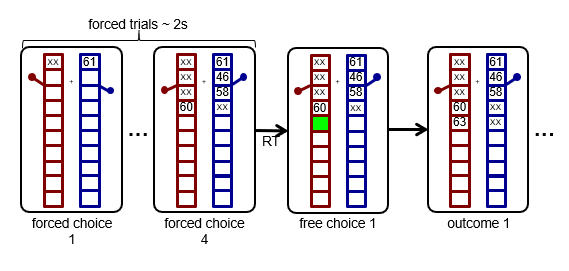
\includegraphics[width=\textwidth]{figures/taskfig1.PNG}
			\caption{Time line of a horizon 6 game.  The game begins with four forced choice trials in which participants are instructed which option to play.   After these forced trials they are free to choose between the two options for the rest of the game (6 trials in this case).
			COMBINE THIS WITH FIGURE 7 FOR TASK CONDITIONS
			CAN YOU MAKE THESE FIGURES LOOK NICER I.E. MORE LIKE MINE?  REDUCE LINE WIDTHS ETC ... IF NOT SEND ME POWER POINTS AND I WILL MAKE INTO PDFS}
			\label{fig:taskfig1}
		\end{center}
	\end{figure}
	
	The first four trials of each game were forced-choice trials, in which only one of the options was available for the participant to choose. We used these forced-choice trials to manipulate the relative ambiguity of the two options, by providing the participant with different amounts of information about each bandit before their first free choice. The four forced-choice trials set up two uncertainty conditions: unequal uncertainty(or [1 3]) in which one option was forced to be played once and the other three times, and equal uncertainty(or [2 2]) in which each option was forced to be played twice. After the forced-choice trials, participants made either 1 or 6 free choices (two horizon conditions). (See Figure \ref{fig:taskfig2})	 
	
	\begin{figure}[H]
		\begin{center}
			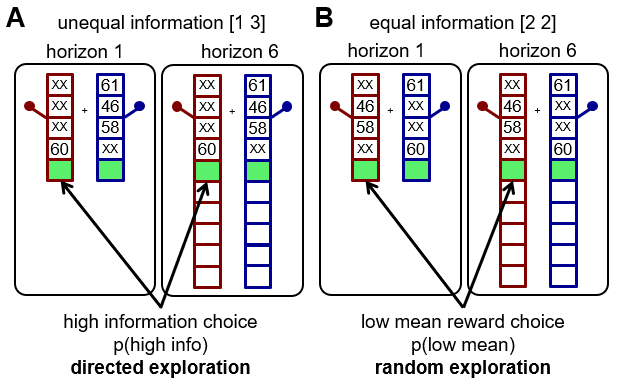
\includegraphics[width=\textwidth]{figures/taskfig2.PNG}
			\caption{Task conditions}
			\label{fig:taskfig2}
		\end{center}
	\end{figure}
	
	%Finally, the random seeds were not perfectly controlled between subjects.  The first 16 subjects ran the task with identical random seeds and thus all 16 saw the same sequence of forced-choice trials in both vertex and RFPC sessions. For the remaining subjects the random seed was unique for each subject and each session, thus these subjects had unique a series of forced-choice trials for each session.  Despite this limitation we saw no evidence of different behavior across the two groups.
	
	\subsection*{Data and code}
	%Behavioral data as well as Matlab code to recreate the main figures from this paper can be found on the Dataverse website at https://dataverse.harvard.edu/dataset.xhtml?persistentId=doi:10.7910/DVN/CZT6EE.
	
	
	\subsection*{Model-based analysis}
	We modeled behavior on the first free choice of the Horizon Task using a version of the logistic choice model in \citep{wilson2014} that was modified to differentiate internal and external noise. In particular, we assume that in repeated games, external noise remains the same whereas internal noise can change. 
	
	\subsubsection*{Hierarchical Bayesian Model}
	
	To model participants' choices on this first free-choice trial, we assume that they make decisions by computing the difference in value $\Delta Q$ between the right and left options, choosing right when $\Delta Q > 0$ and left otherwise.  Specifically, we write
	\begin{equation}
	\Delta Q= \Delta R+A \Delta    I+b+n_{ext}+n_{int}
	\end{equation}
	where, the experimentally controlled variables are $\Delta R=R_{right}-R_{left}$, the difference between the mean of rewards shown on the forced trials, and $\Delta I$, the difference information available for playing the two options on the first free-choice trial. For simplicity, and because information is manipulated categorically in the Horizon Task, we define $\Delta I$ to be +1, -1 or 0, +1 if one reward is drawn from the right option and three are drawn from the left in the [1 3] condition, -1 if one from the left and three from the right, and in [2 2] condition, $\Delta I$ is 0. $n_{ext}$ and $n_{int}$ are external noise and internal noise respectively. 
	
	The other variables are: the spatial bias, $b$, which determines the extent to which participants prefer the option on the right; the information bonus $A$, which controls the level of directed exploration; $n_{ext}$ denotes the external, external noise, which is identical on the repeat versions of each game; and $n_{int}$ denotes internal noise, which is uncorrelated between repeat plays and changes every game.
	
	Each subject's behavior in each horizon condition is described by 4 free parameters: the information bonus $A$, the spatial bias, $b$, the standard deviation of the external noise, $\sigma_{ext}$, and the standard deviation of the internal noise, $\sigma_{int}$ (Table \ref{tab:pars2}, Figure \ref{fig:model}). Each of the free parameters is fit to the behavior of each subject using a hierarchical Bayesian approach \citep{hbm1}.  In this approach to model fitting, each parameter for each subject is assumed to be sampled from a group-level prior distribution whose parameters, the so-called `hyperparameters', are estimated using a Markov Chain Monte Carlo (MCMC) sampling procedure. The hyper-parameters themselves are assumed to be sampled from `hyperprior' distributions whose parameters are defined such that these hyperpriors are broad.  
	
	The particular priors and hyperpriors for each parameter are shown in Table \ref{tab:pars2}. For example, we assume that the information bonus, $A^{is}$, for each horizon condition $i$ and for each participant $s$, is sampled from a Gaussian prior with mean $\mu^{A}_{i}$ and standard deviation $\sigma_{i}^A$. These prior parameters are sampled in turn from their respective hyperpriors: $\mu_{i}^{A}$, from a Gaussian distribution with mean 0 and standard deviation 10, and $\sigma_{i}^A$ from an Exponential distribution with parameters 0.1.
	%\begin{table}[h]
	%	\small
	%	\begin{center}
	%		\begin{tabular}{|c|c|c|c|}
	%			\hline
	%			Parameter &
	%			Horizon dependent? &
	%			Uncertainty dependent? &
	%			Repeated game dependent? \\
	%			\hline
	%			information bonus, $A$ &
	%			yes &
	%			n/a &
	%			no \\
	%			\hline
	%			spatial bias, $B$ &
	%			yes &
	%			no &
	%			no \\
	%			\hline
	%			external decision noise, $\sigma_{ext}$ &
	%			yes & 
	%			yes &
	%			no \\
	%			\hline
	%			internal decision noise, $\sigma_{int}$ &
	%			yes & 
	%			yes &
	%			yes \\
	%			\hline
	%		\end{tabular}
	%	\end{center}
	%	\caption{Model parameters and their dependence on horizon, uncertainty condition and repeated games }
	%	\label{para1}
	%\end{table}%
	
	\begin{table}[h]
		\small
		\begin{tabular}{|c|c|c|c|}
			\hline
			Parameter & Prior & Hyperparameters & Hyperpriors \\
			\hline
			information bonus, $A_{is}$ 
			& $A_{is} \sim $  Gaussian($\mu_i^{A}$, $\sigma_i^{A}$) 
			& $\theta_{i}^{A} = (\mu_i^{A}, \sigma_i^{A}) $
			& \specialcell{
				$\mu_i^{A} \sim $ Gaussian( 0, 100 ) \\ 
				$\sigma_i^{A} \sim $ Exponential(0.1)}		\\
			\hline
			spatial bias, $B_{is}$ 
			& $B_{is} \sim $  Gaussian($\mu_i^{B}$, $\sigma_i^{B}$) 
			& $\theta_{i}^{B} = (\mu_i^{B}, \sigma_i^{B}) $
			& \specialcell{
				$\mu_i^{B} \sim $ Gaussian( 0, 100 ) \\ 
				$\sigma_i^{B} \sim $ Exponential(0.1)}		\\
			\hline
			deviation of external noise, $\epsilon_{isg}$ 
			& $\sigma_{i} \sim $  Gamma($k_i^{ext}$, $\lambda_{i}^{ext}$) 
			& $\theta_{i}^{ext} = (k_i^{ext}, \lambda_i^{ext}) $
			& \specialcell{
				$k_i^{ext} \sim $ Gaussian(0.1) \\ 
				$\lambda_i^{ext} \sim $ Exponential(10)}		\\
			\hline
			deviation of internal noise, $\sigma_{isgr}$ 
			& $\sigma_{is} \sim $  Gamma($k_i^{int}$, $\lambda_{i}^{int}$) 
			& $\theta_{i}^{int} = (k_i^{int}, \lambda_i^{int}) $
			& \specialcell{
				$k_i^{int} \sim $ Gaussian(0.1) \\ 
				$\lambda_i^{int} \sim $ Exponential(10)}		\\
			\hline
		\end{tabular}
		\caption{Model parameters, priors, hyperparameters and hyperpriors. CHECK UPDATE}
		\label{tab:pars2}	
	\end{table}
	
	\subsubsection*{Model fitting using MCMC}
	The model was fit to the data using Markov Chain Monte Carlo approach implemented in the JAGS package \citep{jags} via the MATJAGS interface (psiexp.ss.uci.edu/research/programs\_data/jags). This package approximates the posterior distribution over model parameters by generating samples from this posterior distribution given the observed behavioral data.  
	
	In particular we used 4 independent Markov chains to generate 16000 samples from the posterior distribution over parameters (4000 samples per chain).  Each chain had a burn in period of 2000 samples, which were discarded to reduce the effects of initial conditions, and posterior samples were acquired at a thin rate of 1.  Convergence of the Markov chains was confirmed {\it post hoc} by eye. 
	
	\begin{figure}[H]
		\begin{center}
			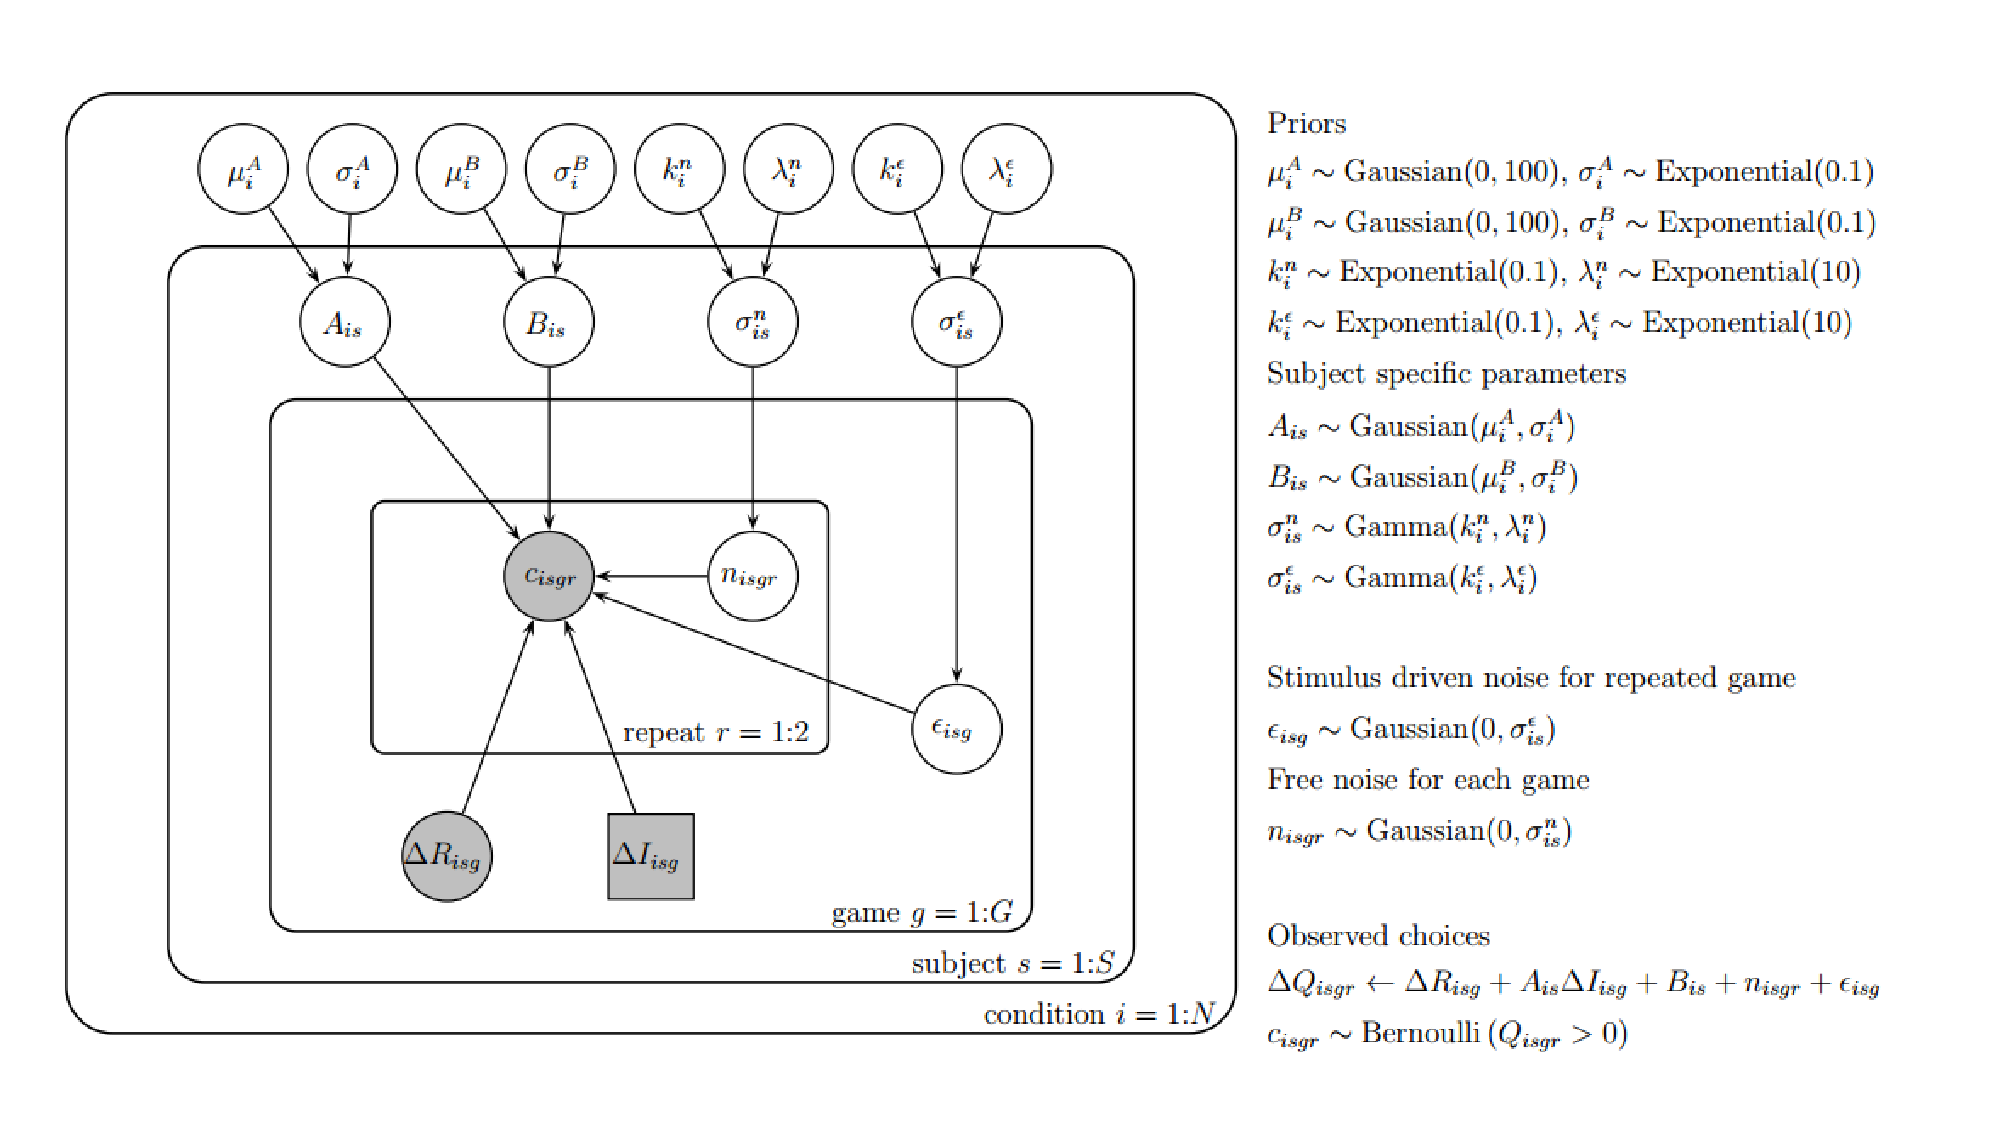
\includegraphics[width=\textwidth]{figures/hbm.pdf}
			\caption{Hierarchical Bayesian model}
			\label{fig:model}
		\end{center}
	\end{figure}
	
	\subsubsection*{Parameter recovery\label{ch:appendix:bayesrecovery}}
	
	To be sure that our fit parameter values were meaningful, we tested the ability of our model fitting procedure to recovery parameters from simulated data.  In particular, we simulated choices with the fitted parameters from the Hierarchical Bayesian analysis, and the re-fit the simulated the choices to see whether we can recover the parameters. 
	
	Results of this parameter recovery procedure are shown in Figure \ref{fig:pararecover1}. As is clear from this figure, parameter recovery is good for all parameters apart from the bias, which is likely due to this parameter being so close to zero (Figure XXX PANEL NUMBER).  The recovery for the noise parameters, $\sigma_{ext}$ and $\sigma_{int}$, is slightly better for horizon 1 than horizon 6. This is because it requires more trials to recover bigger noises, so with the same number of choices it is harder to recover overall bigger noises in horizon 6. In addition we see better recovery for internal noise than external noise because we effectively have half as many trials for external noise since we are only generating one sample of external noise for each repeated game pair. Overall, we are able to recover both external and internal noises using our model to a satisfactory extent.
	
	\begin{figure}[h]
		\begin{center}
			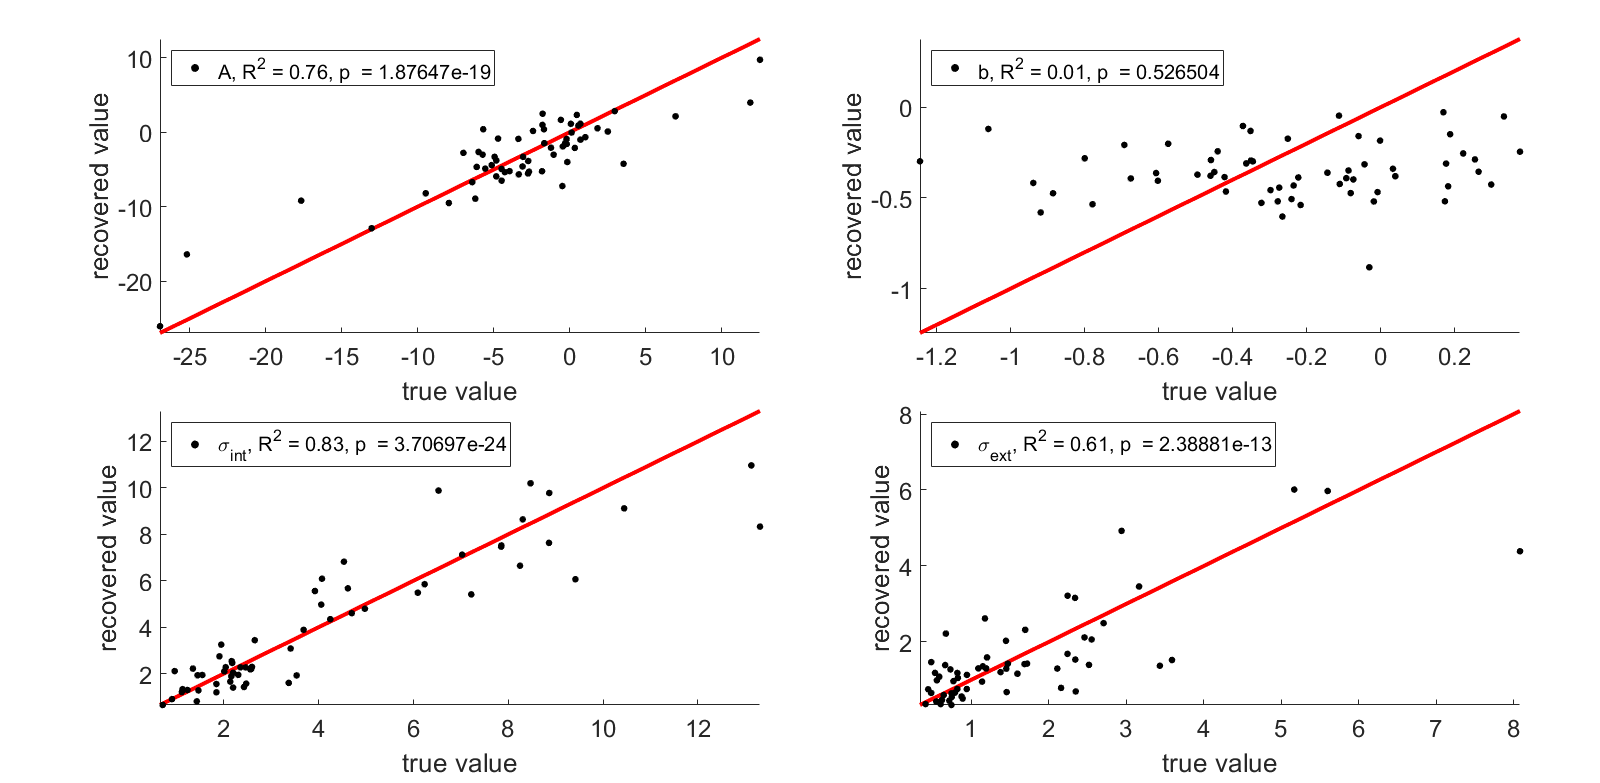
\includegraphics[width=1\textwidth]{figures/paramrecover_1.png}
			\caption{Parameter recovery over the subject-level means of information bonus($A$), spatial bias($b$), internal noise variance($\sigma_{int}$) and external noise variance($\sigma_{ext}$) for horizon 1 games
			COMBINE THESE TWO, HAVE TWO COLUMNS, LEFT IS HORIZON 1, RIGHT IS HORIZON 6.  REDUCE NUMBER OF SIGNIFICANT FIGURES IN p VALUES.  DON'T USE LEGEND, USE TEXT FUNCTION TO PUT TEXT ON PLOTS.  RED LINES CHANGE TO DOTTED BLACK LINES.  
			XLABELS - SIMULATED $A$, YLABELS FIT $A$, I.E. MAKE SPECIFIC FOR EACH PARAMETER
			USE ADDABCS FUNCTION TO ADD ABCs!
			}
			\label{fig:pararecover1}
		\end{center}
	\end{figure} 
	
	\begin{figure}[H]
		\begin{center}
			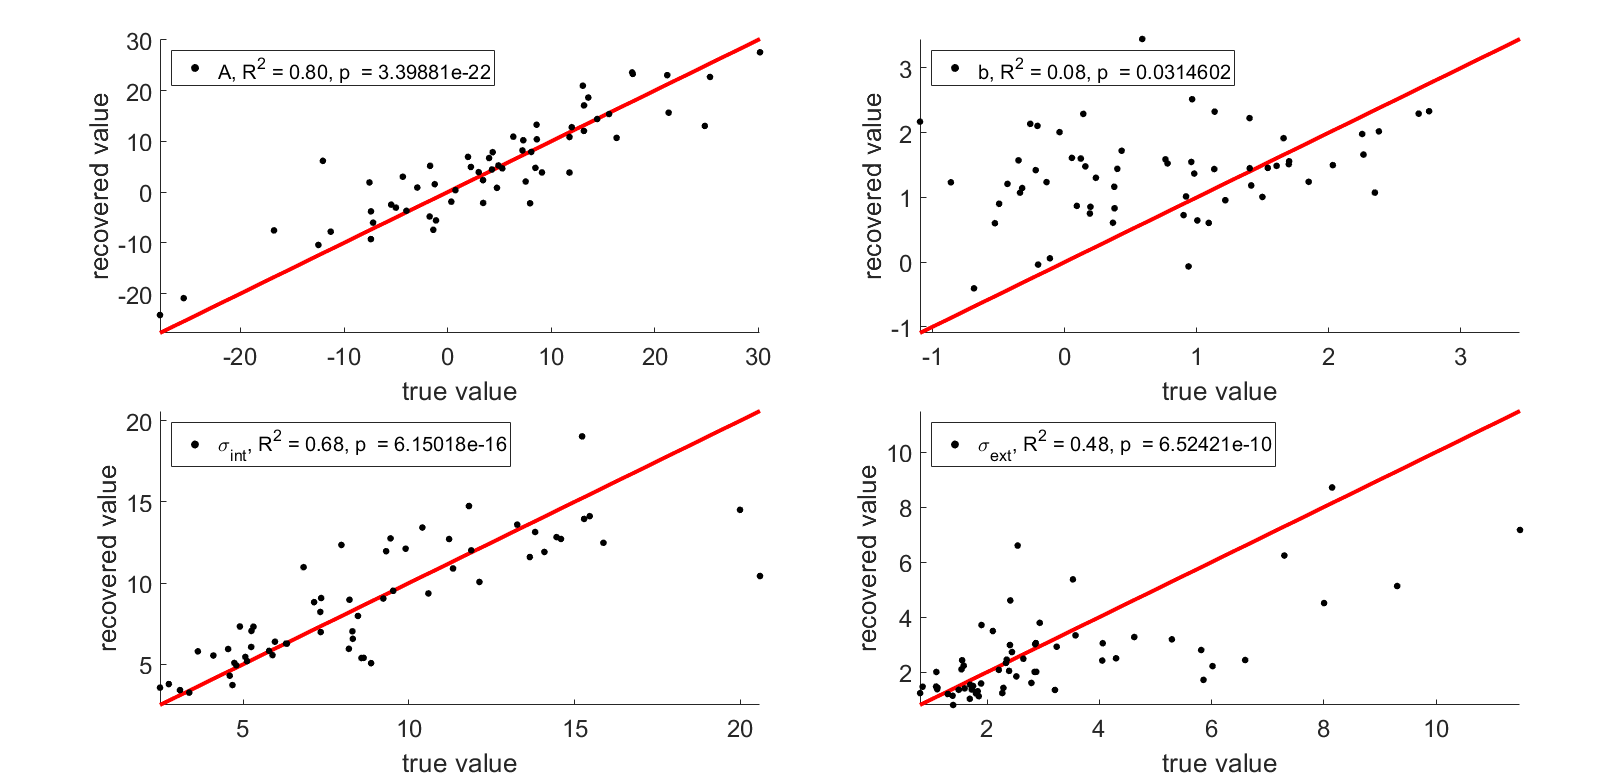
\includegraphics[width=1\textwidth]{figures/paramrecover_2.png}
			\caption{Parameter recovery over the subject-level means of information bonus($A$), spatial bias($b$), internal noise variance($\sigma_{int}$) and external noise variance($\sigma_{ext}$) for horizon 6 games}
			\label{fig:pararecover2}
		\end{center}
	\end{figure}
	%References
	%Plummer, M. (2003, March). JAGS: A program for analysis of Bayesian graphical models using Gibbs sampling. In Proceedings of the 3rd international workshop on distributed statistical computing (Vol. 124, p. 125).
	%Rescorla, R. A., & Wagner, A. R. (1972). A theory of Pavlovian conditioning: Variations in the effectiveness of reinforcement and nonreinforcement. Classical conditioning II: Current research and theory, 2, 64-99.
	
	
	
	
	\bibliographystyle{plainnat}
	%\bibliographystyle{unsrt}
	\bibliography{Refs/refs}
	
	% add the Bibliography to the Table of Contents
	\cleardoublepage
	\ifdefined\phantomsection
	\phantomsection  % makes hyperref recognize this section properly for pdf link
	\else
	\fi
	\addcontentsline{toc}{chapter}{Bibliography}
	


\end{document}
